\documentclass{oblivoir}
\usepackage{graphicx} % Required for inserting images
\usepackage{verbatim}

\usepackage[a4paper, total={6in, 9in}]{geometry}
\hypersetup{
    colorlinks=true,
    linkcolor=blue
}

\title{HW3}
\author{C311054 박민서}
\date{2025년 5월 16일}

\begin{document}

\maketitle

\section{Fuction}
\subsection{함수 정의}
\begin{verbatim}
    external_declaration                                                                           
        : function_definition 
            {funcnt++; /* 함수 정의 카운트 */
            intcnt+=inttmp; charcnt+=chartmp; pocnt+=potmp; arrcnt+=arrtmp;
            inttmp=chartmp=potmp=arrtmp=0;}
        | declaration
        | preprocessor
        ;
    
    function_definition
        : declaration_specifiers declarator compound_statement
        | declarator compound_statement
        ;
\end{verbatim}
함수의 정의는 yacc에서 function\_definition이라는 심볼이다. 이 심볼은 external\_declaration으로 무조건 reduce되기 때문에 이 때 카운트해준다.
함수의 전방선언은 declaration으로 reduce되기 때문에 카운트되지 않는다.

\subsection{함수 사용}
\begin{verbatim}
    postfix_expression
        : primary_expression
        | postfix_expression '[' expression ']'
        | postfix_expression '(' ')' {funcnt++;} /*함수 사용*/
        | postfix_expression '(' argument_expression_list ')' {funcnt++;} /*함수사용*/
        | postfix_expression '.' IDENTIFIER {opcnt++;}
        | postfix_expression PTR_OP IDENTIFIER {opcnt++;}
        | postfix_expression INC_OP {opcnt++;}
        | postfix_expression DEC_OP {opcnt++;}
        ;
\end{verbatim}
함수의 사용은 '함수이름(인자)'의 형태이기 때문에 해당 부분에서 카운트한다.

\section{Operation}
연산자 토큰이 사용되는 곳에서 카운트하면 된다.
\subsection{참조연산자, 후위증감연산자}
\begin{verbatim}
    postfix_expression
        : primary_expression
        | postfix_expression '[' expression ']'
        | postfix_expression '(' ')' {funcnt++;} 
        | postfix_expression '(' argument_expression_list ')' {funcnt++;}
        | postfix_expression '.' IDENTIFIER {opcnt++;} /*참조*/
        | postfix_expression PTR_OP IDENTIFIER {opcnt++;} /*참조*/
        | postfix_expression INC_OP {opcnt++;} /*후위증가*/
        | postfix_expression DEC_OP {opcnt++;} /*후위감소*/
        ;
\end{verbatim}
\subsection{전위증감연산자}
\begin{verbatim}
    unary_expression
        : postfix_expression
        | INC_OP unary_expression {opcnt++;} /*전위증가*/
        | DEC_OP unary_expression {opcnt++;} /*전위감소*/
        | unary_operator cast_expression
        | SIZEOF unary_expression
        | SIZEOF '(' type_name ')'
        ;
\end{verbatim}
\subsection{cast연산자}
\begin{verbatim}
    cast_expression
        : unary_expression
        | '(' type_name ')' cast_expression {opcnt++;} 
        ;
\end{verbatim}
\subsection{산술연산자}
\begin{verbatim}
    multiplicative_expression
        : cast_expression
        | multiplicative_expression '*' cast_expression {opcnt++;}
        | multiplicative_expression '/' cast_expression {opcnt++;}
        | multiplicative_expression '%' cast_expression {opcnt++;}
        ;

    additive_expression
        : multiplicative_expression
        | additive_expression '+' multiplicative_expression {opcnt++;}
        | additive_expression '-' multiplicative_expression {opcnt++;}
        ;
\end{verbatim}
\subsection{비트연산자}
\begin{verbatim}
    shift_expression
        : additive_expression
        | shift_expression LEFT_OP additive_expression {opcnt++;}
        | shift_expression RIGHT_OP additive_expression {opcnt++;}
        ; 
        
    and_expression
        : equality_expression
        | and_expression '&' equality_expression {opcnt++;}
        ;

    exclusive_or_expression
        : and_expression
        | exclusive_or_expression '^' and_expression {opcnt++;}
        ;

    inclusive_or_expression
        : exclusive_or_expression
        | inclusive_or_expression '|' exclusive_or_expression {opcnt++;}
        ;
\end{verbatim}
\subsection{논리연산자}
\begin{verbatim}
    relational_expression
        : shift_expression
        | relational_expression '<' shift_expression {opcnt++;}
        | relational_expression '>' shift_expression {opcnt++;}
        | relational_expression LE_OP shift_expression {opcnt++;}
        | relational_expression GE_OP shift_expression {opcnt++;}
        ;

    equality_expression
        : relational_expression
        | equality_expression EQ_OP relational_expression {opcnt++;}
        | equality_expression NE_OP relational_expression {opcnt++;}
        ;
\end{verbatim}
\subsection{관계연산자}
\begin{verbatim}
    logical_and_expression
        : inclusive_or_expression
        | logical_and_expression AND_OP inclusive_or_expression {opcnt++;}
        ;

    logical_or_expression
        : logical_and_expression
        | logical_or_expression OR_OP logical_and_expression {opcnt++;}
        ;
\end{verbatim}
\subsection{대입연산자}
\begin{verbatim}
    assignment_expression
        : conditional_expression
        | unary_expression assignment_operator assignment_expression {opcnt++;}
        ;

    assignment_operator
        : '='
        | MUL_ASSIGN
        | DIV_ASSIGN
        | MOD_ASSIGN
        | ADD_ASSIGN
        | SUB_ASSIGN
        | LEFT_ASSIGN
        | RIGHT_ASSIGN
        | AND_ASSIGN
        | XOR_ASSIGN
        | OR_ASSIGN
        ;
\end{verbatim}
모든 대입연산자는 assignment\_operator로 reduce되기 때문에 assignment\_operator가 reduce되는 곳에서 한번만 세면 된다.




\section{Int, Char, Pointer, Array}

조건이 많아서 까다로운 부분이었다. 조건은 다음과 같다.


-변수의 갯수는 포인터가 1개일 때는 카운트, 2개 이상이면 카운트하지 않는다.


-배열에서 변수도 카운트한다.


-함수의 파라미터에서도 카운트한다. 단, 전방 선언에서는 중복으로 세지 않도록 해야 한다.


-함수의 리턴값에서는 세지 않는다.


-포인터함수에서는 포인터와 함수만 세고 변수는 세지 않는다. \newline \newline


이 조건들을 구분해내기 위해 direct\_declarator부분에서 각 종류에 따라 심볼 값을 할당했다.
\begin{verbatim}
    declarator
        : pointer direct_declarator     {if($1==1)$$=$2+5;else $$=$2+10;}
        | direct_declarator             {$$=$1;}
        ;
    
    direct_declarator
        : IDENTIFIER                                    {$$=0;}
        | '(' declarator ')'                            {if($2>=5)$$=1;else $$=$2;}
        | direct_declarator '[' constant_expression ']' {$$=2;}
        | direct_declarator '[' ']'                     {$$=2;}
        | direct_declarator '(' parameter_type_list ')' {if($1==1)$$=4;else $$=3;}        
        | direct_declarator '(' identifier_list ')'     {$$=0;}
        | direct_declarator '(' ')'                     {if($1==1)$$=4;else $$=3;}
        ;
    pointer
        : '*'                                   {$$=1;}
        | '*' type_qualifier_list               {$$=1;}
        | '*' pointer                           {$$=$2+1;}
        | '*' type_qualifier_list pointer       {$$=$3+1;}
        ;
\end{verbatim}
direct\_declarator의 심볼 값에서
0은 식별자, 2는 배열, 3은 함수를 나타낸다.
1과 4는 포인터함수를 처리하기 위한 값인데,
먼저 declarator를 보자. 
declarator는 pointer의 심볼 값(*의 갯수를 나타내도록 되어있음)을 보고
direct\_declarator에 포인터가 1개 붙으면 direct\_declarator의 심볼 값에 5를 더하고 포인터가 2개 이상이면 10을 더한다. 
포인터가 없으면 direct\_declarator의 심볼 값을 그대로 갖는다.
direct\_declarator의 심볼 값은 0부터 4까지 있기 때문에 5와 10을 더하면 모든 값들이 다른 수로 구분된다.


만약 direct\_declarator의 2번째 규칙에서 괄호 안 declarator의 심볼 값이 5이상이라면 포인터가 하나이상 있다는 것이고 이 상태를 심볼 값 1로 나타낸다. 포인터가 없는 경우는 기존 심볼 값을 그대로 사용한다. 


direct\_declarator의 5번째와 7번째 규칙은 함수를 나타내는데 이 때 규칙안의  direct\_declarator부분이 심볼 값 1을 갖는다면 전체 구조는 (* direct\_declarator)( 파라미터 )가 되므로 포인터함수가 된다. 포인터 함수는 심볼 값 4로 나타낸다.

declarator가 가질 수 있는 심볼 값은 다음과 같다.
\begin{figure}[h]
    \centering
    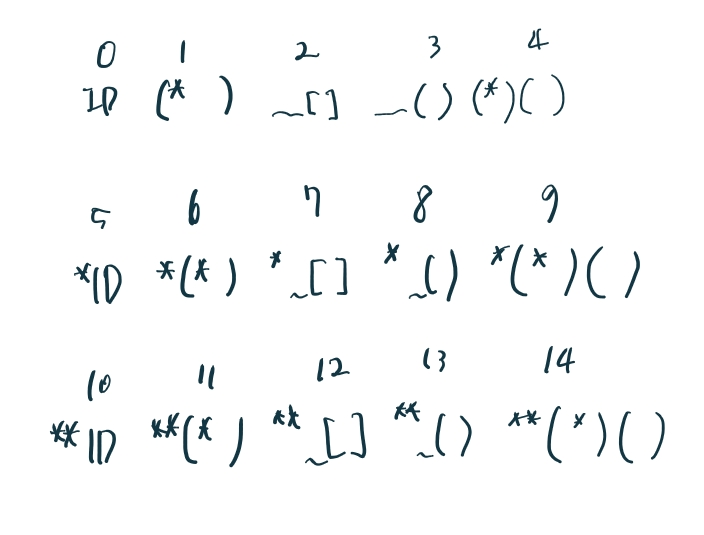
\includegraphics[width=0.8\linewidth]{declarator_value.jpg}
    \caption{declarator symbol value}
    \label{fig:fig1}
\end{figure}

declarator가 reduce되는 곳은 init\_declarator, struct\_declarator, parameter\_declaration, function\_definition 이렇게 네 개이다.

\subsection{parameter\_declaration}
parameter\_declaration을 먼저 보겠다.
\begin{verbatim}
    parameter_declaration
        : declaration_specifiers declarator
        {
        if($2==0||$2==1||$2==2||$2==5||$2==7)
                {
                if($1==2)chartmp++;if($1==4)inttmp++;
                }
        if($2==1||$2==5||$2==6||$2==7||$2==10||$2==11||$2==12) potmp++;
        if($2==2||$2==7||$2==12) arrtmp++;
        }
        | declaration_specifiers abstract_declarator
        | declaration_specifiers
        ;
\end{verbatim}

그림 \ref{fig:fig1}을 보면 변수는 0,1,2,5,7에서 카운트, 포인터는 1,5,6,7,8,10,11,12에서 카운트, 배열은 2,7,12에서 카운트해야한다. 마지막 2열은 함수이므로 카운트에서 제외한다. 변수는 declaration\_specifiers의 심볼 값에 따라 int,char 각각 세어준다.

parameter\_declaration은 함수의 정의에 들어갈 수도 있고 전방선언에 들어갈 수도 있다.
만약 전방선언이 된다면 파라미터에서 변수, 포인터, 배열 모두 카운트하면 안된다. 따라서 이 가능성을 염두하고 바로 카운트값을 올리는 대신 tmp라는 별개의 변수로 세어놓는다.

translation\_unit은 external\_declaration의 반복이고 external\_declaration에는 function\_definition과 declaration만 존재한다. 함수의 전방선언은 declaration으로 reduce되고 함수의 정의는 function\_definition으로 reduce된다. 따라서 이 둘 중 하나로 결정되는 external\_declaration에서 tmp값을 cnt에 더해줄 수 있다.


\subsection{function\_definition}
\begin{verbatim}
    external_declaration
        : function_definition 
            {funcnt++; 
            intcnt+=inttmp; charcnt+=chartmp; pocnt+=potmp; arrcnt+=arrtmp;
            inttmp=chartmp=potmp=arrtmp=0;}
        | declaration
        | preprocessor
        ;

    function_definition
        : declaration_specifiers declarator compound_statement
        | declarator compound_statement
        ;

\end{verbatim}
declarator가 function\_definition으로 reduce될 경우는 함수의 리턴값이기 때문에 이 때는 세지 않는다. 

\subsection{init\_declarator}
\begin{verbatim}
    init_declarator
        : declarator
        {
        chartmp=0; inttmp=0; arrtmp=0; potmp=0;
        $$=0;
        if($1%5==4) funcnt++;
        if($1!=0&&$1!=2&&$1%5!=3) pocnt++;
        if($1==0||$1==1||$1==2||$1==5||$1==7) $$=1; 
        if($1%5==2) arrcnt++;
        }
        | declarator '=' initializer
        {opcnt++;
        chartmp=0; inttmp=0; arrtmp=0; potmp=0;
        $$=0;
        if($1%5==4) funcnt++;
        if($1!=0&&$1!=2&&$1%5!=3) pocnt++;
        if($1==0||$1==1||$1==2||$1==5||$1==7) $$=1;
        if($1%5==2) arrcnt++;
        }
        ;
\end{verbatim}
declarator가 parameter\_declaration이 아닌 다른 곳으로 reduce된 경우는 tmp의 값을 0으로 초기화해준다.
함수의 파라미터가 아닌 일반 선언에서는 변수의 갯수를 바로 세지 않고 변수를 셀 수 있는지 여부를 심볼 값으로 전달한다. (\$\$가 1이라는 것은 변수로 카운팅 가능함을 알린다.) 이는 아직 변수의 타입을 모르기 때문이고, int a,b와 같은 여러 변수를 동시에 한번에 선언할 때의 카운팅도 가능하게 한다.
함수,포인터,배열의 갯수는 바로 세어준다.

\begin{verbatim}
    init_declarator_list
        : init_declarator                               {$$=$1;}
        | init_declarator_list ',' init_declarator      {$$=$1+$3;}
        ;
\end{verbatim}
init\_declarator\_list의 심볼 값은
init\_declarator 심볼 값의 1의 갯수를 세도록 되어있다.

\begin{verbatim}

    declaration_specifiers
        : storage_class_specifier                               {$$=0;}
        | storage_class_specifier declaration_specifiers        {$$=$2;}
        | type_specifier                                        {$$=$1;}
        | type_specifier declaration_specifiers                 {$$=$1;}
        | type_qualifier                                        {$$=0;}
        | type_qualifier declaration_specifiers                 {$$=$2;}
        ;
        
    type_specifier
        : VOID          {$$=1;}
        | CHAR          {$$=2;}
        | SHORT         {$$=3;}
        | INT           {$$=4;}
        | LONG          {$$=5;}
        | FLOAT         {$$=6;}
        | DOUBLE        {$$=7;}
        | SIGNED        {$$=8;}
        | UNSIGNED      {$$=9;}
        | struct_or_union_specifier     {$$=10;}
        | enum_specifier        {$$=11;}
        | TYPE_NAME     {$$=12;}
        ;
\end{verbatim}

declaration\_specifiers는 type\_specifier값을 전달해준다.
type\_specifier의 심볼 값은 종류 별로 다른 값을 갖는다.

\begin{verbatim}
    declaration                                                                                      
    : declaration_specifiers ';'                                             
    | declaration_specifiers init_declarator_list ';' 
        {if($1==4)intcnt+=$2; if($1==2)charcnt+=$2;}
    | TYPEDEF declaration_specifiers init_declarator_list ';'
        {
        if($2==4)intcnt+=$3; if($2==2)charcnt+=$3;
        typedef_li[typedef_cnt++]=name;
        }
        ;
\end{verbatim}

declaration\_specifiers와 init\_declarator\_list가 만나는 지점인 declaration에서 declaration\_specifiers의 심볼 값으로 타입을 파악하고 init\_declarator\_list의 값 만큼 카운트한다.

\subsection{struct\_declarator}
\begin{verbatim}
    struct_declaration
        : specifier_qualifier_list struct_declarator_list ';' {if($1==4)intcnt+=$2; if($1==2)charcnt+=$2;}
        ;

    specifier_qualifier_list
        : type_specifier specifier_qualifier_list       {$$=$1;}
        | type_specifier                                {$$=$1;}
        | type_qualifier specifier_qualifier_list       {$$=$2;}
        | type_qualifier                                {$$=0;}
        ;

    struct_declarator_list
        : struct_declarator                             {$$=$1;}
        | struct_declarator_list ',' struct_declarator  {$$=$1+$3;}
        ;

    struct_declarator
        : declarator
                {
                chartmp=0; inttmp=0; arrtmp=0; potmp=0;
                $$=0;
                if($1%5==4) funcnt++;
                if($1!=0&&$1!=2&&$1%5!=3) pocnt++;
                if($1==0||$1==1||$1==2||$1==5||$1==7) $$=1;
                if($1%5==2) arrcnt++;
                }
        | ':' constant_expression               {$$=-1;}
        | declarator ':' constant_expression
                {
                chartmp=0; inttmp=0; arrtmp=0; potmp=0;
                $$=0;
                if($1%5==4) funcnt++;
                if($1!=0&&$1!=2&&$1%5!=3) pocnt++;
                if($1==0||$1==1||$1==2||$1==5||$1==7) $$=1;
                if($1%5==2) arrcnt++;
                }
        ;
\end{verbatim}
구조체에서는 일반 선언문과 동일하다.

\section{조건문, 반복문}
\begin{verbatim}
    statement
        : labeled_statement
        | compound_statement
        | expression_statement
        | selection_statement   {selcnt++;}
        | iteration_statement   {loopcnt++;}
        | jump_statement
        ;
\end{verbatim}
조건문은 selection\_statement, 반복문은 iteration\_statement이므로 그대로 세면 된다.

\section{리턴문}
\begin{verbatim}
    jump_statement
        : GOTO IDENTIFIER ';'
        | CONTINUE ';'
        | BREAK ';'
        | RETURN ';'            {retcnt++;}
        | RETURN expression ';' {retcnt++;}
        ;
\end{verbatim}
리턴문은 RETURN 토큰이 쓰인 곳에서 세어준다.

\section{변수의 선언 위치}
\begin{verbatim}
    compound_statement
    	: '{' '}'
    	| '{' statement_list '}'
    	| '{' declaration_list '}'
    	| '{' declaration_list statement_list '}'
    	;
    declaration_list
    	: declaration
    	| declaration_list declaration
    	;
    
    statement_list
    	: statement
    	| statement_list statement
    	;
\end{verbatim}
이것은 기존의 ANSI C Yacc 문법이다. declaration\_list와 statement\_list의 순서가 정해져 있기 때문에 변수의 전방선언만 허용된다.

\begin{verbatim}
    compound_statement
        : '{' '}'
        | '{' declaration_statement_list '}'
        ;

    declaration_statement_list
        : declaration
        | declaration declaration_statement_list
        | statement
        | statement declaration_statement_list
        ;

\end{verbatim}
위와 같이 declaration과 statement의 순서가 무엇이든 허용되도록 고쳤다.

\begin{verbatim}
    iteration_statement
        : WHILE '(' expression ')' statement
        | DO statement WHILE '(' expression ')' ';'
        | FOR '(' expression_statement expression_statement ')' statement
        | FOR '(' expression_statement expression_statement expression ')' statement
        | FOR '(' declaration expression_statement ')' statement
        | FOR '(' declaration expression_statement expression ')' statement
        ;
\end{verbatim}
또한 for문의 괄호 안에서도 선언이 가능하도록 아래 두 줄을 추가했다.


\section{typedef}
\begin{verbatim}
    declaration
        : declaration_specifiers ';'
        | declaration_specifiers init_declarator_list ';' {if($1==4)intcnt+=$2; if($1==2)charcnt+=$2;}
        | TYPEDEF declaration_specifiers init_declarator_list ';'
                {
                if($2==4)intcnt+=$3; if($2==2)charcnt+=$3;
                typedef_li[typedef_cnt++]=name;
                }
        ;
\end{verbatim}
기존의 storage\_class\_specifier에 있던 TYPEDEF 토큰을 처리하기 위해 declaration에 옮겨 따로 규칙을 추가했다.
typedef 안에서 명시적으로 선언된 변수도 카운팅을 해주고 typedef\_li의 typedef\_cnt 인덱스에 타입의 이름을 넣어준다.

\begin{verbatim}
    int check_type()
    {
        name=strdup(yytext);
        if(is_typedef(yytext)) return TYPE_NAME;
        else if(is_define(yytext)) return CONSTANT;
        else return IDENTIFIER;

    }
\end{verbatim}

name은 lex에서 식별자(가 아닐 수도 있는 문자와 숫자의 조합)의 타입을 검사할 때 그 식별자의 이름을 복사한 값이다.
typedef로 선언되었는지를 검사하고 맞다면 TYPE\_NAME 토큰을 반환한다. 

\begin{verbatim}
    extern char*name;
    char*typedef_li[100];
    int typedef_cnt=0;
    
    int is_typedef(char*s){
        for(int i=0;i<typedef_cnt;i++){
                if(strcmp(s,typedef_li[i])==0)return 1;
        }
        return 0;
    }
\end{verbatim}
yacc파일에서는 lex에서 선언된 name을 받아주고 is\_typedef함수에서 typedef\_li를 순회하면서 일치하는 이름이 있는지 검사한다.

\section{define}
\begin{verbatim}

"define"                { return(DEFINE);}

"#"                     { return('#'); }
\end{verbatim}
lex에 위와 같은 규칙을 추가하였다.

define의 경우 typedef와 유사하게 처리한다.
\begin{verbatim}
    char*define_li[100];
    int define_cnt=0;
    int is_define(char*s){
        for(int i=0;i<define_cnt;i++){
                if(strcmp(s,define_li[i])==0)return 1;
        }
        return 0;
    }
\end{verbatim}
\begin{verbatim}
    define_constant
        : '#' DEFINE IDENTIFIER CONSTANT {define_li[define_cnt++]=name;}
        ;
\end{verbatim}
마지막 파라미터가 상수인 경우만 처리했다.
\begin{verbatim}
    int check_type()
    {
        name=strdup(yytext);
        if(is_typedef(yytext)) return TYPE_NAME;
        else if(is_define(yytext)) return CONSTANT;
        else return IDENTIFIER;

    }
\end{verbatim}
lex에서 타입검사 시 define으로 할당되어 있는 값이라면 CONSTNAT 토큰으로 반환해준다.

\section{include}

\begin{verbatim}
    "include".*"\n"         { return(INCLUDE); }
\end{verbatim}

\begin{verbatim}
    preprocessor
        : define_constant
        | '#' INCLUDE
        ;
\end{verbatim}
\begin{verbatim}
    external_declaration
        : function_definition 
        {funcnt++; 
        intcnt+=inttmp; charcnt+=chartmp; pocnt+=potmp; arrcnt+=arrtmp; 
        inttmp=chartmp=potmp=arrtmp=0;}
        | declaration
        | preprocessor
        ;
\end{verbatim}

위와 같이 include와 define도 파싱이 되도록 수정했다.

\section{주석}
\begin{verbatim}
    "/*"                    { comment(); }
    "//".*"\n"              {;}
\end{verbatim}
\begin{verbatim}
    void comment()
    {
            char c, c1;
    
    loop:
            while ((c = input()) != '*' && c != 0);
    
            if ((c1 = input()) != '/' && c != 0)
            {
                    unput(c1);
                    goto loop;
            }
    
    }
\end{verbatim}
주석은 위와 같이 처리하였다. lex의 규칙은 longest matching을 기본으로 하지만 주석은 shorest matching을 해야한다. 그렇지 않으면 주석을 여러개 사용했을 때 그 사이에 끼어있는 일반 코드가 주석처리될 수 있기 때문이다. shorest matching을 정규표현식으로 처리하는 것은 어렵기 때문에 기존의 comment함수를 이용했다. 그리고 출력은 되지 않도록 putchar는 지웠다. 

\end{document}